\documentclass[11pt]{article}
\usepackage{amsmath, amssymb, amscd, amsthm, amsfonts}
\usepackage{graphicx}
\usepackage{enumitem}
\usepackage{hyperref}
\usepackage{ragged2e}
\usepackage{listings}
\usepackage{caption,subcaption}
\usepackage{float}
\graphicspath{ {images/} }

\oddsidemargin 0pt
\evensidemargin 0pt
\marginparwidth 40pt
\marginparsep 10pt
\topmargin -20pt
\headsep 10pt
\textheight 8.7in
\textwidth 6.65in
\linespread{1.2}

\title{Emulating Cloud Environment using Virtualization}
\author{Arshdeep Singh \and Prayag Panta \and Pradeep Parajuli \and Rajesh Jha}
\date{}

\begin{document}

\maketitle

\begin{abstract}
This dissertation aims to analyse the impact of various clients on the cloud server simulated via Virtualization tools such as VMWare and Virtual Box. This report contains several parameters such as Throughput, CPU usage etc. which will be used to describe the performance of the cloud.
\end{abstract}

\section{Introduction}\label{section-introduction}
First step for simulating the Cloud Environment is Virtualization. VMWare and Virtual Box were used for this. 

These two approaches are mentioned which are used for this assignment.

\begin{enumerate}
  \item LAMP stack for Server setup and Python for analytics
  \item ReactJS and NodeJS for server setup and Plotly API for analytics
\end{enumerate}

\section{Methodologies}\label{methodologies}

\subsection{LAMP stack and Python}
\subsubsection{Server Setup}
PHP script is used to enter data from the user and to measure throughput along with resource uses statistics.\par
\vspace{.5em}
\justifying
    Front-end comprised of a form where user was provided with an option to enter name, email along with corresponding number of entries to be made in the database. Upon submitting the form, User is directed to a page where is notified the corresponding number of successes and failures along with resource usage statistics. In case of server shutdown, user is notified with an alert the server is down at the moment.\par

    \vspace{.5em}
    For Server these methods are defined for getting \textit{CPU usage} and \textit{Memory Usage}.
        \begin{itemize}
            \item \textbf{get\_server\_memory\_usage}:
                This function uses \textit{free} command executed via \textit{shell\_exec} function available in PHP. \textit{free} command shows the total memory usage of the system at the given moment. Then \textit{Trim} function is used to remove white spaces from the output. Total and active memory usage is extracted from the output to calculate the memory usage percentage at the given moment.
        
                \begin{figure}
                \centerline{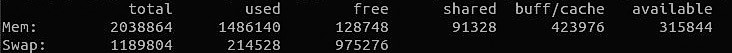
\includegraphics[scale=.75]{memory-usage.jpeg}}
                \caption{Sample output for memory usage}
                \end{figure}
        
            \item \textbf{get\_server\_cpu\_usage}:
                To calculate the CPU usage \textit{sys\_getloadavg} command is used. This shows system load average over the last second.
                Output is in form of array as shown below:
                Array \newline
                \{
                    \begin{enumerate}[label={[\arabic*]}]
                    \item 65.34
                    \item 68.23
                    \item 72.34
                    \end{enumerate}
                \} \newline
                First element of this array is taken to get current cpu usage.
        \end{itemize}
        
        When form is submitted by the user, resource usage and timestamp are recorded in the file namely success.txt and failure.txt. Data is entered in former only when there is a successful entry in the database, for all other cases entry is made in latter. \par
        
        Connection to backend database is made for entering the data. \textit{\textbf{Mariadb}}
        database is used to store the data. 
        % There is a table named "cl" with this as its configuration.
        % \begin{enumerate}
        %     \item \textbf{RN} int(11) primary key
        %     \item \textbf{NAME} varchar(50)
        %     \item \textbf{EMAIL} varchar(80)
        % \end{enumerate} 
\subsubsection{Analysis}
Python script is used to analyse two files success.txt and failure.txt. For each timestamp frequency is calculated for each entry in the file. Using this frequency we calculate Throughput of the server. 
It is calculated for 10,000 enteries in each case. It is mapped on the graph for following cases and conclusions are drawn from it.
\begin{enumerate}
    \item Single Client and Single Server
    \item Multiple Client and Single Server
    \item Multiple Client and Multiple Server
\end{enumerate}

\subsection{ReactJS, NodeJS and Plotly}
\subsubsection{Server Setup}
Using ReactJS front-end server is setup on port 3000 of localhost. This is accessed by User. 
This page contains table which shows enteries of the \textbf{\textit{products}} table present in database. User enters product name, its price and number of enteries to store in the database. As the user submits \textbf{\textit{Add Products}} button this will shoot a fetch request to backend server which is at port 4000 of localhost. \par

This also contains various states to store the current cached data in the session. These are following states.
\begin{enumerate}
    \item \textbf{products} Products store the enteries from the database table to show it on the webpage.
    \item \textbf{product} To store product details written by user in that session.
    \item \textbf{count} To store the number of enteries entered by user.
\end{enumerate}

In backend, NodeJS server is setup using \textbf{expressjs} which is a web application framework provided by NodeJS. This is on port 4000 of localhost. This establishes a connection with database and incase of error throws error. To calculate CPU usage and throughput two functions are used.
\begin{enumerate}
    \item \textbf{throughputLogger} To calculate throughput for each request comping to server \textit{current time} is stored in \textbf{\textit{requests}} array. For every successful response for the entry in the database, items are updated in the requests array. Now this array is used in throughputLogger function to calculate throughput. For each timeframe for 1000 milliseconds we repeat this procedure again and again to calculate throughput for each second.
    
    \begin{lstlisting}
    function throughputLogger() {
        var now = new Date();
        var aMinuteAgo = now - (1000);
        var cnt = 0;
        // since recent requests are at the end of the array, search the array
        // from back to front
        for (var i = requests.length - 1; i >= 0; i--) {
            if (requests[i] >= aMinuteAgo) {
                ++cnt;
            } else {
                break;
            }
        }
        yData.push(cnt);
        xData.push(now.getMinutes() + ':' + now.getSeconds());
        console.log("Throughput: ", cnt)
    	setTimeout(throughputLogger, 1000)  
    };
    \end{lstlisting}
    
    \item \textbf{cpuLogger} To calculate the total CPU usage at that moment first we loop through all of its cores then for each core total time each core tick is stored as \textit{totalTick} and idle time is stored as \textit{totalIdle}. Both of these are divided by total number of cores to get average value for each core. These values are calculated at two times seperated by small interval. Difference of pervious value and current value of total and idle are stored in \textit{totalDiff} and \textit{idleDiff} respectively. CPU usage is logged in console using this formula
    
    \begin{lstlisting}
        samples[i] = (1 - idleDiff / totalDiff);
    \end{lstlisting}
\end{enumerate}

These endpoints are used to facilitate the working of backend server.\textbf{\textit{MySQL}} query is executed for showing and adding product. Graph is plotted via \textbf{\textit{Plotly}} API.
\begin{enumerate}
    \item \textbf{/products} GET request to show list of products present in database.
    \item \textbf{/products/add} POST request to add a product in the database.
    \item \textbf{/graph} GET request to signal server thread to call plotly API and plot graph corresponding to throughput calculated.
\end{enumerate}

\section{Analysis}\label{analysis}
Results of different approaches gives these graphs as shown below.

\begin{figure}[H]
    \centering 
    \begin{subfigure}{0.40\textwidth}
      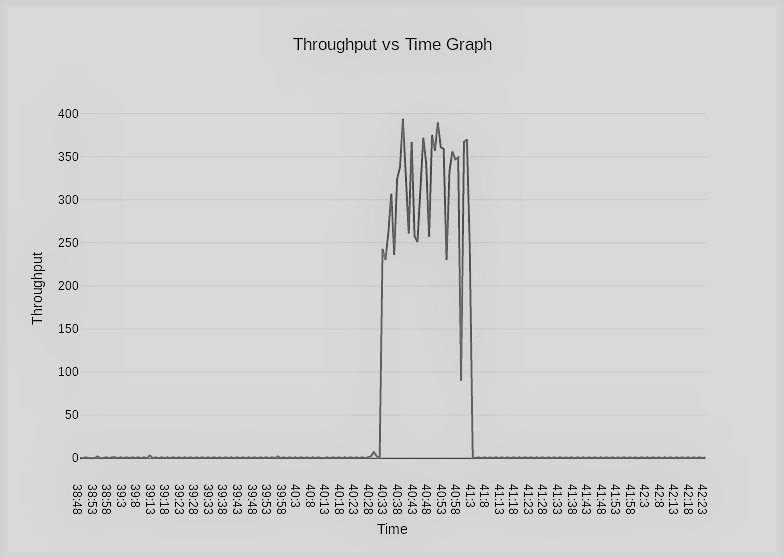
\includegraphics[width=\linewidth]{1-1}
      \caption{Single Client vs Single Server}
      \label{fig:1}
    \end{subfigure}
    \hfil
    \begin{subfigure}{0.40\textwidth}
      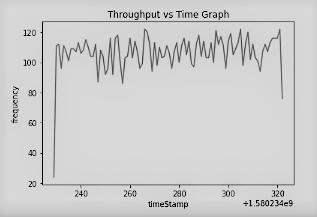
\includegraphics[width=\linewidth]{2-1}
      \caption{Single Client vs Single Server}
      \label{fig:4}
    \end{subfigure}
    \medskip
    \begin{subfigure}{0.40\textwidth}
      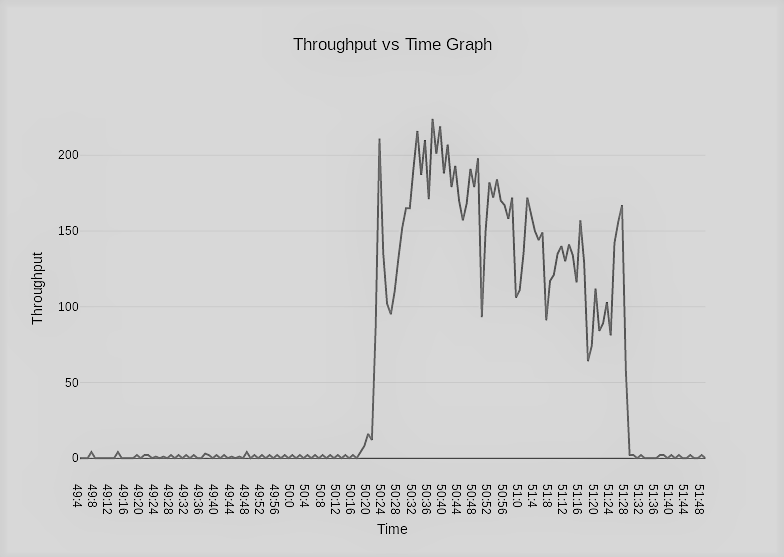
\includegraphics[width=\linewidth]{1-2}
      \caption{Multiple Client vs Single Server}
      \label{fig:2}
    \end{subfigure}
    \hfil
    \begin{subfigure}{0.40\textwidth}
      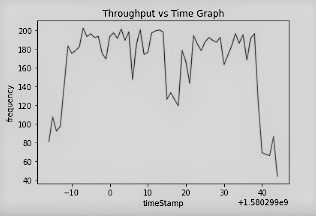
\includegraphics[width=\linewidth]{2-2}
      \caption{Multiple Client vs Single Server}
      \label{fig:5}
    \end{subfigure}
    \medskip
    \begin{subfigure}{0.40\textwidth}
      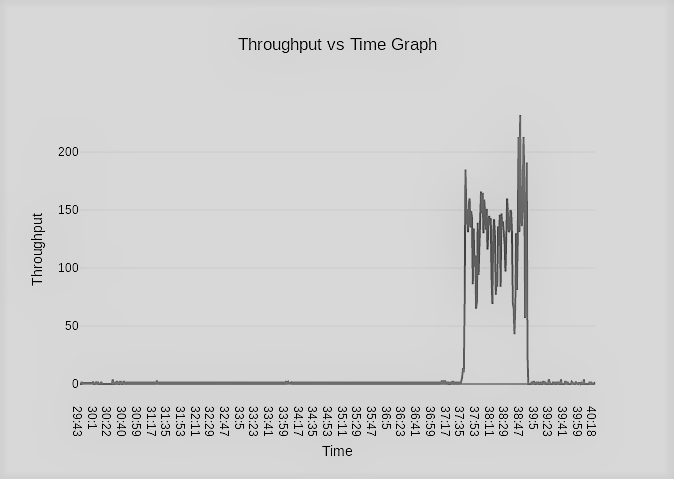
\includegraphics[width=\linewidth]{1-3}
      \caption{Multiple Client vs Multiple Server}
      \label{fig:3}
    \end{subfigure}
    \hfil
    \begin{subfigure}{0.40\textwidth}
      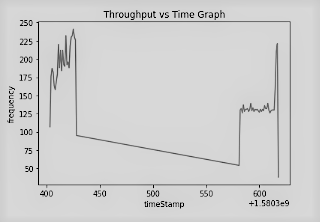
\includegraphics[width=\linewidth]{2-3}
      \caption{Multiple Client vs Multiple Server}
      \label{fig:6}
    \end{subfigure}
\caption{Throughput output of 2 Approaches}
\label{fig:images}
\end{figure}

Figures on each side in every row represent threshold function vs time graph of different approach. These demonstrate 3 possible scenarios. Following are the possible conclusions drawn from according to us.
\begin{itemize}
    \item In First case, throughput reaches to almost 400 but in subsequent cases when number of clients is increased which in our case is doubled from 1 to 2. The value of throughput is decreased to approximately 200. Therefore threshold is inversely proportional to number of clients in the cloud. \par
    \centering
        Threshold $\propto$ 1/Number of Clients
    \item In Second case the time taken to complete more than first case which is due to multiple clients are requesting server in the same time which leads to formation of queue of requests which need to be served after completion of first ones. Also, the memory consumption also increases and threshold is low which leads to increase in time. Therefore time taken to respond to client is directly proportional to number of clients. \par
    \centering
        Time taken to respond to client $\propto$ Number of Clients.
    \item In all of the above cases, there is a dip in threshold after some time of execution of the client's requests. This is due to excessive use of memory which is above that server can easily provide to clients. Decrease in memory and increase in CPU usage leads to huge decrease in threshold value. This criterion is used for server shutdown and reset conditions in bash script.
\end{itemize}
Another bash cron script is run which checks after some interval that our Memory usage has not succeeded the threshold which is determined checking these conditions/scenarios. In the case when memory usage is excessive, shutdown of server and reset of server is initiated.

\section{Conclusion}\label{conclusion}
While simulating a cloud environment using Virtualization in a personal computer we have drawn these conclusions.
\begin{enumerate}
    \item Increasing load on cloud server decreases threshold. As the number of clients requesting read and write requests increases, the amount of successful responses of those requests decreases and takes longer time to respond.
    \item Distributing resources in server (3rd scenario) leads to delay in response and low threshold. As memory and CPU of virtual server are shared by another virtual server running in same machine leads to this result.
    \item Server goes to low state and cannot supply enough threshold to each client which leads to longer loading times which further leads to larger bounce rate as user does not the response in reasonable time.
    \item As virtual machines are made on personal computers, they are not easy to simulate crash scenario when large number of clients are simultaneously requesting the server for I/O operations. Disk space is large so enough data entries to crash is also not possible in reasonable amount of time.
    \item Advance controlling of virtual environment like creation and destruction of VM on its own is not possible in free versions of VMware and Virtual Box. These were limiting factors for fully simulating cloud environment.
\end{enumerate}

\section{Source Code}\label{source-code}
\begin{enumerate}
    \item \href{https://github.com/PrayagPanta/Throughput-Measurement-using-PHP}{Approach-1}
    \item \href{https://github.com/ArshdeepSingh98/Virtual-Client-Server}{Approach-2}
\end{enumerate}

\end{document}
